\documentclass[11pt]{article}

\usepackage{fullpage}
\usepackage[ruled,vlined,linesnumbered]{algorithm2e}
\usepackage{graphicx}
\graphicspath{ {.} }

\begin{document}
\setcounter{secnumdepth}{2}

\title{
  C Project - Final Report \\
  \large ARM Assembler and Extension}
\author{Group 9\\\\Carlos Valencia Vargas, Mihnea Gogu,\\Madi Baiguzhayev and Alex Constantin-G\'omez}

\maketitle

\section{ARM Assembler}
\subsection{Structure}
We decided that it would be logical to divide the work in the same way we did for the emulator, since each of us already had a good understanding of the different instruction types we were respectively assigned to implement in the emulator: Carlos worked on the parser and the multiply instruction, Mihnea worked on the branch instruction, which involved keeping track of labels in a symbol table, and, Alex and Madi worked on the single data transfer and data processing instructions respectively.
\\\\
The file structure of the assembler is consistent with the emulator's structure: an \texttt{assemble.c} file with the \texttt{main()} function which opens both the input and output files and calls the appropriate functions from the code within the \texttt{assembler/} directory. Again, for consistency, there is a source and header file that generates the binary code for each of the four different instruction types. The \texttt{parser.\{c,h\}} contains the code that implements the one pass assembler and calls the functions from the other files in the directory. Any commonly used utility functions are written in \texttt{asm\_utilities.\{c,h\}}. We also defined a \texttt{type\_defs.h} header file which defines common structs and enums used throughout the code. Since we also required the use of dynamic data structures, we implemented a hash table in \texttt{hash\_table.\{c,h\}}, a linked list in \texttt{list.\{c,h\}} and an array list in \texttt{array\_list.\{c,h\}}.

\subsection{Implementation}
We decided to challenge ourselves by implementing the one-pass algorithm, which is supposedly less straightforward than the two-pass algorithm suggested in the specification.\\\\
Our implementation relied on two main data structures: a hash table to keep track of labels (the symbol table), and a list structure for storing instructions and for keeping track of offsets which cannot be set until the end of the pass. We decided to implement both a doubly linked list and an array list for these purposes. \\\\
The implementation of our one-pass assembler (located in \texttt{parser.c}) is summarised in pseudocode in the table below (Algorithm 1). 

\begin{algorithm}
\SetAlgoLined
initialise the symbol table\;
initialise the instruction list\;
\ForEach{line in the asm file}{
    tokenise the instruction (line)\;
    decode the instruction using the tokens\;
    try to add labels to branch instructions with labels not yet defined\;
    \eIf{instruction is a label}{
        add label to symbol table\;
        ensure the label points to the next non-label instruction on the next iteration\;
    }{
        add the instruction to the instruction list\;
    }
}
check branch instructions with not yet defined labels\;
calculate any remaining offsets for the relevant LDR instructions\;
write instruction bytes to binary file\;
free all used data structures and resources\;
\caption{One Pass Assembler}
\end{algorithm}

One of the challenges involved in writing a one-pass assembler other than keeping track of labels is calculating the offsets for \texttt{LDR} instructions, where bytes of data need to be written at the end of the binary file. Calculating the offset bits requires the address of the final instruction, however because there is only one pass through the file, you cannot know this until the end. To solve this, we used a list of \texttt{LDR} instructions which have not yet had their offset bits set, their index (line number) and a list of the bytes that have to be written at the end. This allowed us to set the offset bits at the end of the pass without having to iterate through all of the instructions again. The function implementing this is called \texttt{calculate\_pending\_offsets()}, located in \texttt{parser.c} and is called in the assembler algorithm (line 15 of Algorithm 1).

\section{Extension: ARM GUI Debugger}
\subsection{Description}
Our extension is a graphical user interface debugger for ARM11 programs that runs within the terminal. It is inspired by GDB and our aim was to make it easy and intuitive to use. Its main features are listed below and can be seen in Figure \ref{fig:debugger}:

\begin{itemize}
    \item Setting breakpoints at addresses and pausing execution when they are reached
    \item Single instruction stepping
    \item User-friendly display of registers and memory contents
    \item The current instruction is highlighted in the memory map
    \item Print contents in hexadecimal, binary and decimal of any memory address and register
    \item Help box with a list of all available commands
    \item Displays the history of output messages
\end{itemize}

\begin{figure}
    \centering
    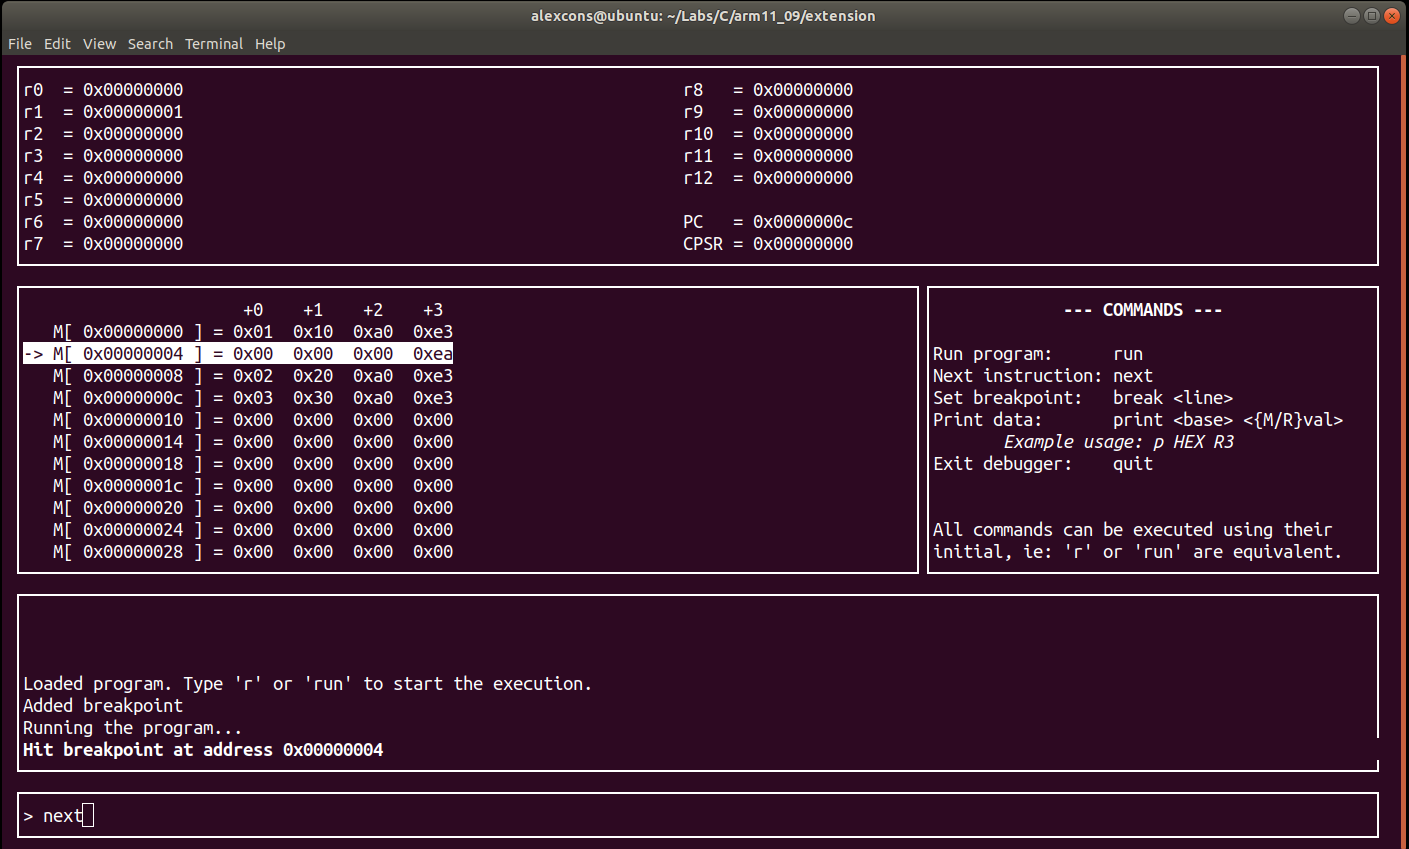
\includegraphics[width=0.8\textwidth]{debugger}
    \caption{A screenshot of the debugger in action}
    \label{fig:debugger}
\end{figure}

\subsubsection{Example usage}
In order to run the debugger, you need to specify what binary file you would like to execute as a single command-line argument. This will clear your terminal screen and render the GUI with the file's bytes loaded into memory. You are then free to input any of the commands in the prompt at the bottom of the interface. To run the program, you can type \texttt{run}. To set a breakpoint, you can type \texttt{break <address>}. To step to the next instruction, you can type \texttt{next}. To print the contents of a register, you can type \texttt{print <BASE> <{M/R}value>}, where you can specify the base to be \texttt{HEX}, \texttt{BIN} or \texttt{DEC}. In the second argument, you must specify a leading \texttt{M} for a memory address or \texttt{R} for a register, followed by the address/name. For example, \texttt{print BIN R4} will print the contents of register 4 in binary. Also, any command can be executed using its initial, i.e.: \texttt{run} and \texttt{r} are equivalent, like in GDB.

\newpage
\subsection{Implementation overview}
The implementation of the debugger was divided into two parts: creating a graphical user interface for the user to interact with (the frontend) and adapting/modifying the existing emulator code to support the features described above (the backend).
\\\\
For the frontend, one of our objectives was to make the program easy and intuitive to use, so we decided to create the GUI within the terminal. We ended up using the Ncurses library, which usually comes pre-installed on most Linux distributions. It provides a high-level API for building text-based applications within the terminal. We decided to represent each window/subregion on the screen with our own custom defined structs, which contain attributes related to the window. For example, we created an \texttt{OutputWin} struct which contains the window itself (of type \texttt{WINDOW}) provided by Ncurses and the history of past output messages. We followed this convention for all the different regions on the screen and it made our code much more readable and structured.\\
We also wrote a few functions for parsing user input and checking if the user entered a valid command supported by the program.
\\\\
For the backend, since our debugger had to run ARM11 binary files, we reused the emulator code but tweaked it to support a \textit{debugging mode}. We reused the hash table from our assembler to store any breakpoints. Moreover, we passed three extra parameters into the \texttt{start\_pipeline()} function which is the entry point for starting the emulator. We made a \texttt{bool} pointer to identify if we were running the emulator in \textit{debugging mode}, as this would imply reading input from the user via the GUI function \texttt{get\_user\_input()} defined in \texttt{extension/gui.c}. Likewise, we passed the breakpoints hash table and another \texttt{bool} pointer. This pointer was due to the dual mode nature of the code execution, as sometimes we needed the code to be executed without interruption until the next breakpoint (the \texttt{run} command) and sometimes stepping to the next instruction (the \texttt{next} command) regardless of breakpoints.

\subsection{Implementation challenges}
One of the biggest challenges was to find and learn a library for creating graphical programs. This involved researching and experimenting with, in our case, Ncurses by writing small programs to familiarise ourselves with its API and to identify what features were going to be viable to implement in the given timeframe. We used the online manual pages for Ncurses and other resources we could find to overcome this challenge.\\\\
Another obstacles we faced was splitting the work equally such that Linux users could work on and test the GUI frontend, while non-Linux users would work on the backend.\\
With regard to the backend, we also had to make sure that when adapting the emulator code we didn't break it. Of course, with careful use of Git we managed to overcome this. For every incremental change, we made sure that the emulator would still compile and pass the tests as it did before.

\newpage
\subsection{Testing}
Testing our debugger was another fairly challenging task. Since it is GUI program designed for human usage, any form of automated testing was not a viable option due to the short amount of time we had. Therefore, we relied on manual testing, which involved running the many of the already provided ARM11 binary files and making sure all the features we implemented were working as expected. All four members tested the program so that there were more chances of finding bugs.

\subsubsection{Effectiveness of our testing}
The biggest advantage we had when it came to testing is that we could reuse the wide range of test cases (assumed to be correct) as part of the provided test suite for the emulator and assembler. This allowed us to test our program several times and at the same time, it also let us know that our emulator was still working correctly.\\
The downside to the way we tested was of course the fact that it was all manual. This made it long and tedious, and it may not have been very reliable since it depends on human input (which may imply errors when testing, such as forgetting to try a certain command).

\section{Reflection and final thoughts}
\subsection{Group Reflection}
We worked in a group effectively by allocating clear tasks for each person to do and by making sure to communicate daily on progress. Our way of communicating was using a WhatsApp group for text messaging quick updates and issues that we were aiming to resolve, and then a Discord group that we use for video calls to share our screens. Every time we had the task of merging our work together into master, we had a video call where one person shares their screen while merging to ensure we did it correctly. A few times we did pair programming such as for the emulator instructions which was useful for avoiding errors.\\ 
Moreover, when it came to discussions of design implementations and work allocations, we had voice calls to figure it out. Our way of allocating work was efficient by how we played to our strengths - for instance, implementing the same type of instruction we did for the emulator for the assembler. Each person chose what they were comfortable and confident in doing. Our text chats helped too for when we had questions regarding other member's parts.\\
If we were to work again next time, we would keep the same level of communication since it is crucial to good group work. We think having only one chat service in use would be more fruitful for organization and simplicity. Also, it would be simpler if we all used the same operating system so there are no compatibility issues (although we worked around this).

\subsection{Individual Reflections}
In addition to our group reflection, below are the individual reflections by all four group members.

\subsubsection{Carlos Valencia Vargas}
Overall, I think I’ve adapted well to the project and most importantly it has been a great learning experience. Having had regular group meetings has made it easy to separate the workload equally, without depending on someone else’s code. We committed to Git after finishing each small section and commented it out appropriately to allow the other members to understand it. Personally, I had compatibility problems since I was using a different system to Linux but I managed to find the tools to overcome it and when possible chose to do the part that could be done in any OS. This is something I will change for the future. Also, learning Git better is something positive I will take away from this project. I have also carried out the pair programming technique with other members from the team allowing more ideas and quick solutions/help to be found on the spot. Finally, we have kept to a strict format and structure for the code as this is truly helpful when programming as a group and have adapted the code to easily merge everyone's part.

\subsubsection{Mihnea Gogu}
The group project went smooth, we split all the tasks equally and effectively and had regular calls whenever we merged multiple branches into master. Each of us worked at more than just one feature, switching from implementing instruction decoding/encoding to prototyping the next task as well as organizing the whole project. Everyone did their part and helped the others. It was a very practical experience of working in a group and the progress was steady and we could definitely see the teamwork having effect, we had virtually no merge conflicts (except an occasional extra comment written in a file or so) and we communicated well.\\
There were no problems regarding team organization, which enabled us to dedicate time fully to implementing all the tasks. Overall I would say the project was a good starting experience for what is to come in the next years, be it at university or in other projects.

\subsubsection{Madi Baiguzhayev}
I think I did my allocated parts well and made sure to get them functional in time so as to not hold other people up. However, in hindsight, I think I should have looked back over my code in order to ensure the code was clear and concise. I found I struggled to contribute ideas and instead found I naturally am better working in supporting roles rather than leader roles. In future group projects, I will try to communicate my opinions more, as I was not assertive sometimes in discussions which is necessary in group work to find which idea is best to take forward. 

\subsubsection{Alex Constantin-G\'omez}
I found that this project was good experience for several reasons. From a technical point of view, it allowed me to practise all the concepts I learned during the C programming lectures and also, I learned how to use Git for collaborative projects, which will probably be an essential skill for future group projects at university and in industry. Another positive that I will take away is that I improved my communication and organisation skills. This helped me fit in well in the group and I think it was one of my strengths. I also think that regular breaks helped me cope throughout the project, for example, resting day or two after completing the emulator. This is something I will look to maintain for future projects, so that I can stay focused during the time I am actually programming.\\
Overall, I am happy with how everything went considering it was my first group programming project and I believe we did a good job.

\end{document}
